\documentclass[12pt]{article}
\usepackage{sydewkrpt}

\begin{document}

\waterlootitle{Design of an American Sign Language Teaching Tool}{

  }{
  Jennifer Blight  20347163\\
  Sara Greenberg 20356941\\
  4B Systems Design Engineering\\
  April 2014
  }

\pagenumbering{roman}

\tocsection{Executive Summary}
American Sign Language (ASL) presents a significant difficulty for those wishing to learn it as
a second language. Due to it’s nature as a visual language, no automated translation tools currently exist that do not require an extensive physical setup. Therefore, we propose an application of existing video preprocessing, feature extraction, and classification methods towards a computer teaching tool to aid those studying ASL to practice in their own homes. 
	
We chose the Microsoft Kinect as a visual input device as it is an affordable, accessible device for which a sizable number of open-source libraries are available. It is also a potential asset for future iterations as the new Kinect set for release in summer 2014 may enable reliable hand- and finger-tracking. In the mean time, we have created simple cloth gloves that allow the collection of data describing the shape and trajectory of a user’s hands. These gloves have coloured markers indicating the fingertips of each hand
	
Through colour thresholding and smoothing filters we extract elements describing the convex hull containing the fingertip markers, one for each hand. During the evolution of the project, we also extracted two centroids, each  representing the position of a hand. This data makes up a vector of features for one video frame.
	
The first prototype classified static ASL signs only, using Support Vector Machines. For later prototypes, a new library of ten dynamic ASL signs was chosen and classified using Hidden Markov Models. A large amount of samples were collected, and this data was used to create on Hidden Markov Model for each sign, as well as a composite model that serves as a detection threshold. For a user’s attempt at a sign to be accepted as correct, the likelihood that their attempt belongs to the Hidden Markov Model in question must exceed the detection threshold.
	
A simple user interface for a flashcard vocabulary game has been created to demonstrate the use of the system. In this game, the user is prompted to perform a random sign from the library. A sliding window technique is used to detect the user’s attempt. When the user has correctly performed the sign, the user is given positive feedback and is prompted to perform a new sign.
	
This system has great potential as an affordable tool for those looking to learn ASL, however there are some modifications necessary before it becomes commercially viable. Adaptive colour thresholding would allow continuous use of the system without interruption due to lighting changes in the user’s environment. Additional features may be required in order to expand the sign database further, as some signs are very similar except with regard to their placement with respect to the user’s face. In such cases, face detection may be a valuable feature. In order to accommodate all users, the gloves must either become available in multiple sizes, or be replaced by skeletal tracking of the user’s bare hands. A more comprehensive user interface would be necessary to engage and entertain the user, and detailed feedback may be more encouraging. Lastly, collecting data is a long and tedious process that had the potential to be accomplished through activities completed by the user to record new sign samples and manually classify samples submitted by other users. 


\newpage

\onehalfspacing
\tableofcontents
\newpage
\doublespacing
\addcontentsline{toc}{section}{\listtablename}
\listoftables
\addcontentsline{toc}{section}{\listfigurename}
\listoffigures
\newpage

\pagenumbering{arabic}
\section{Background}
American Sign Language (ASL) has a unique syntax and grammar, and presents a significant difficulty to learn as a second language. As a result, there is a significant barrier for hearing people to interact with non-hearing people. Most hearing people are unaware of Deaf culture, an oversight that can be partially attributed to having no knowledge of the most common sign language in North America. This ignorance can lead to misunderstandings and unintended injustices.

Automated translation between ASL and English has not been accomplished at the level of translation between popular spoken languages. This can be attributed to the relative difficulty of digitally capturing and processing visual data at high speeds in real time. Recognition of various sign languages is a major area of research, however, current technologies represent only partial solutions to the sign language recognition problem. Additionally, a simple translation system does not allow new users to be immersed in a new culture, but merely acts as a middleman. 

Learning ASL is difficult for a number of reasons: there is no available two-way dictionary. Most learning must occur in a classroom, as it is difficult to practice with no conversation partner. In fact, there are currently no distance-learning tools that provide feedback to the student. 

\subsection{State of the Art}
The problem of sign language recognition and translation has received a lot of attention from researchers in the past few decades as a potential application of gesture recognition algorithms. As a result, there is a great deal of literature describing potential methods for recognizing signs and signed phrases. Most of these methods represent only partial solution--for example, they may recognize gross arm movements or static hand postures but not both--and as of this writing none have been successfully implemented commercially. A sample of these will be described here.

Examples of vision-based systems include a recent project from the University of Waterloo. The goal was to create a desktop video communication application that would allow ASL users to communicate with non-ASL users with a sign-to-text feature. This feature was implemented using a Bayesian classifier to identify skin pixels and an AdaBoosted Haar classifier to identify hand postures. This method is limited to static signs, such as the ASL alphabet, and exhibits limited accuracy.

Another interesting research project is the ASL teaching game for children, CopyCat, from the Georgia Institute of Technology. \cite{Zafrulla} Users wear coloured gloves with wrist-mounted accelerometers and sign in front of a camera in order to direct the characters of a puzzle-solving game. The game uses Hidden Markov Models to verify short, structured ASL sentences of three to five signs based on the accelerometer data as well as the red and blue histograms from the camera (to detect the red and purple gloves). This demonstrates the feasibility of using computer vision techniques to help learners practice sign language. However, the current setup of the system would make it difficult to adopt in the home; lighting and positioning of the user must be carefully controlled and the user is required to wear wrist-mounted accelerometers. 

Furthermore, a recent project developed by Microsoft Research Asia and the Institute of Computing Technology at the Chinese Academy is capable of translating certain sentences of Chinese Sign Language and American Sign Language using the Microsoft Kinect. \cite{Chai} This application creates a 3D trajectory of the user’s hand motions and compares it to a gallery of prototype signs, selecting the most likely candidate based on Euclidean distance. The system has demonstrated recognition rates of 83\%. This project also contains a “Communication” mode, where an avatar can perform sign language motions based on a textual input. The goal of this project is to assist ASL users in their interactions with computers and gaming systems. The drawback of this system is the lack of individual finger tracking. The hands are tracked as points, and so much information is lost. Some signs have similar hand motions but different hand poses and finger motions; for example, the signs “MORE” and “SWEETHEART” are similar, as shown in Figure \ref{fig:MORE}. 

\begin{figure}[h!]
  \centering
  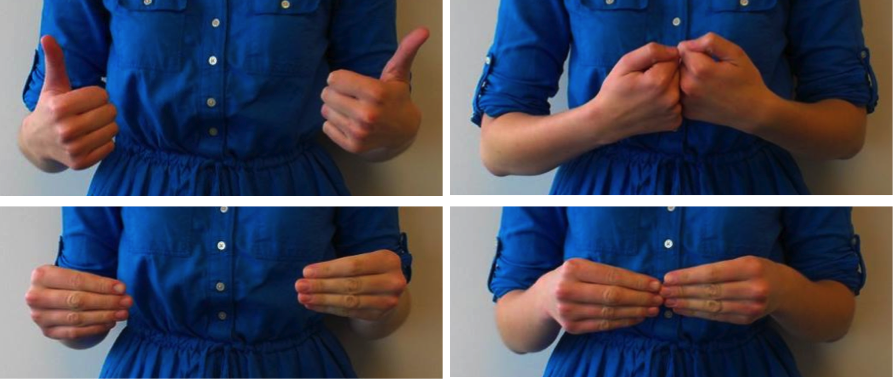
\includegraphics[scale=1]{MORESWEETHEART.png}
  \caption[Example of Signs with Similar Motion]
  { Example of Signs with Similar Motion.  \\ Top: SWEETHEART, Bottom: MORE  }
  \label{fig:MORE}
\end{figure}

The above examples represent only a small sampling of approaches that have been taken to solve the problem. Other techniques used for ASL recognition include Bayesian networks, \cite{Shira} neural networks, \cite{Oz} support vector machines \cite{Agarwal} and several examples of Hidden Markov Models. \cite{Elmezain}\cite{Moni} Some have also attempted to incorporate non-manual markers, small gestures of the face, eyebrows and shoulders meant to convey grammar and context, using face detection and computer vision techniques. \cite{Liu}

\newpage
\section{Problem Statement}
We propose the use of video recognition techniques for the development of a teaching tool intended to train new ASL learners in vocabulary and grammar. Such a problem represents one possible specific application of ASL-to-English video translation which we believe is well-scoped for the time given because we can more easily put constraints on the video content and environment. We will investigate various gesture recognition techniques, alone and in concert, for the purpose of identifying correctly signed gestures and sequences performed by the user. Potential users of the system include Hearing learners and users of other sign languages who want to learn ASL. 

\subsection{Project Goals and Objectives}
Our main goal is to demonstrate the technical feasibility of an ASL teaching tool. From this perspective, our main objectives are to build a classification system that could reliably function as the backend to such a tool and provide an interface by which other developers could create applications. As a secondary objective, we would also construct a simple vocabulary game, to demonstrate the potential of the platform.

\begin{table}[h]
\centering
\caption{Design Objectives}
\label{obj}
\begin{tabular}{|l|p{15cm}|}
\hline
\multicolumn{1}{|c|}{\textbf{\#}} & \multicolumn{1}{|c|}{\textbf{Description}} \\ \hline
O.1 & Create a classification model that is accurate and robust                                                        \\ \hline
O.2 & Create an API for using the classification model and an example application of the API in a teaching application \\ \hline
\end{tabular}
\end{table}

\subsection{Summary of Proposed Design Solution}
Using computer vision and machine learning techniques, we believe we have created an affordable, accessible system that would allow a user to practice ASL in their own home.

The design solution uses simple gloves that allow the capture of features describing the shape and trajectory of the users hands. These features are captured by the Kinect camera, and are used to train a Hidden Markov Model for each sign in the library. A composite model is also generated to create a detection threshold.

The sample game created for this project uses the models to recognize user interaction. A user is prompted to perform a sign, and a sliding window technique monitors the camera feed for signs. An attempt is evaluated based on how likely it is that the attempt belongs to the hidden Markov Model, and if it is more likely that it belongs to the Markov model than the threshold model. If so, the user is given positive feedback.

\subsection{Summmary of Design Requirements}
Tables \ref{require} and \ref{constrain} contain a complete list of design requirements and constraints respectively. 

\begin{table}[h]
\centering
\caption{Design Requirements}
\label{require}
\begin{tabular}{|l|p{15cm}|}
\hline
\multicolumn{1}{|c}{\textbf{\#}} & \multicolumn{1}{|c|}{\textbf{Description}} \\ \hline
R.1 & The video frame must encompass the body parts and surrounding area used when signing, i.e. the signer’s hands, head and shoulders. \\ \hline
R.2 & The method used to capture the location and position of the signer’s hands must function for the speed at which a typical ASL user signs. \\ \hline
R.3 & Hardware necessary to run the solution should be typical or inexpensive and easy to acquire. Either a user could be expected to already own the necessary hardware (example: commonplace laptop and webcam) or the required hardware is on the market and within the financial range of a middle-class person (example: Kinect or Leap Motion sensors). \\ \hline
R.4 & Classification should be near real-time. Lag should not impede user engagement. \\ \hline
R.5 & The solution should correctly identify signs with a 80\% success rate. \\ \hline
R.6 & The solution should function in all common household lighting conditions without loss of speed or accuracy \\ \hline
\end{tabular}
\end{table}

\begin{table}[h]
\centering
\caption{Design Constraints}
\label{constrain}
\begin{tabular}{|l|p{15cm}|}
\hline
\multicolumn{1}{|c}{\textbf{\#}} & \multicolumn{1}{|c|}{\textbf{Description}} \\ \hline
C.1 & Limited time; the project must be completed by March, 2014, while group members have additional obligations for courses and extracurriculars. \\ \hline
C.2 & Small group size; two group members. \\ \hline
C.3 & Limited previous experience of both group members with American Sign Language. \\ \hline
C.4 & Limited previous experience of both group members with feature extraction methods, classification methods, and state-of-the art. \\ \hline
\end{tabular}
\end{table}


\newpage
\section{Engineering Design}
\subsection{Evolution of Design Solution}
The project requires a process described in Figure \ref{process}.  User input is the act of a user performing ASL, which is captured by some form of hardware. A video preprocessing method is implemented to edit the raw data to a more useful format. Feature extraction methods are used to extract relevant information- in this case, this could be the location, shape, or trajectory of the users hand. The information extracted will depend on what sign classification method is used to determine which sign the user has performed. This result is then displayed back to the user in some form.

\begin{figure}[h!]
  \centering
  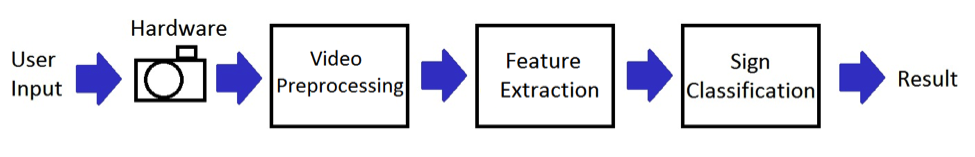
\includegraphics[scale=1]{Process.png}
  \caption{Breakdown of Sign Classification Process}
  \label{process}
\end{figure}

Within our scope, the four main subproblems were 1) the hardware used to collect raw data, 2) the video preprocessing methods, 3) feature extraction methods and 4) the sign classification methods. These areas underwent several iterations during the development of three prototypes. 

\subsubsection{Prototype \#1}
The first prototype was developed during the Fall 2013 semester and was presented at the Dragon’s Den event at the end of November. Hardware and preprocessing techniques were determined, and an initial set of features was chosen.  As the first prototype, classification only focused on a few selected static signs.

\paragraph{Hardware}
The hardware chosen for this project must be inexpensive and readily available to the user, while also providing sufficient data for robust classification. Two options were considered as a visual input device: a generic webcam and the Microsoft Kinect. The Kinect was chosen initially in anticipation of using some of the Kinect's additional features, such as the depth sensor or the hand and face detection libraries. Though more expensive than a webcam, it is a commonly owned device. 

\paragraph{Glove Design and Preprocessing}
We chose to use gloves with coloured markers to simplify the problem of hand detection. A simple, solid-colour knit glove was selected for the glove base and coloured markers were sewn to the fingertipts. The initial and final design of the gloves is shown in Figure \ref{glove_design}. The centre marker on the palm up was not included.

\begin{figure}[h!]
  \centering
  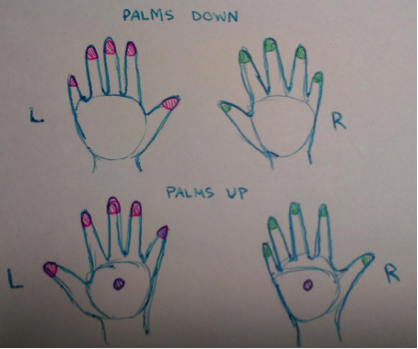
\includegraphics[scale=1]{GloveDesign.png} \qquad
  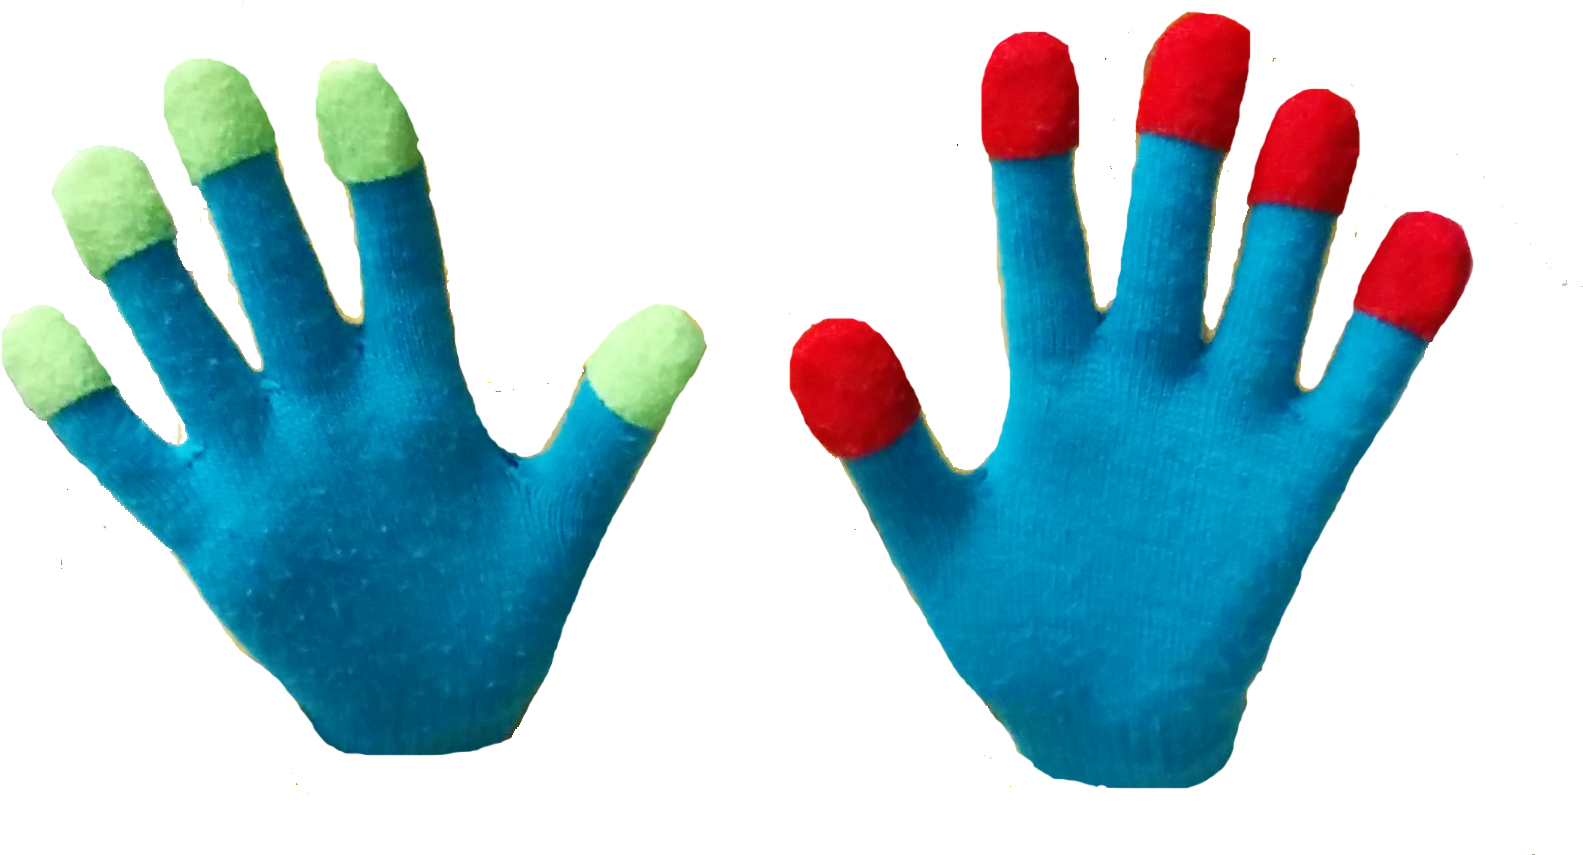
\includegraphics[scale=0.15]{Gloves.png}
  \caption{Initial and Final Glove Design}
  \label{glove_design}
\end{figure}

The final colours for the gloves and markers were selected so as to be highly distinguishable from each other and from the background. The system detects the markers according to predefined thresholds in the YCbCr colourspace. Several denoising and hold-filling filters are applied to the resulting binary image to create smooth blobs.

Due to changes in lighting, the optimal thesholds for distinguishing the markers was highly dependent on the environment. A manual calibration process was developed to quickly determine the appropriate thresholds. Using the calibration script, the user is presented with a frame from a recording and manually selects a section of the appropriate colour. The script then estimate thresholds based on the distribution of pixel values within that section. This process must be repeated everytime to lighting changes or the Kinect is moved to a new location.

\paragraph{Feature Extraction}
In this prototype, only the convex hull of the fingertip markers was extracted as a feature. The binary image produced by preprocessing the Kinect video contains several blobs representing the location of the user’s fingertips. The convex hull is the smallest shape that contains all of the marker blobs but also has no convexity defects along its perimeter. The result is a single shape that describes the relative positions of all the fingers visible in the frame.

\begin{figure}[h!]
  \centering
  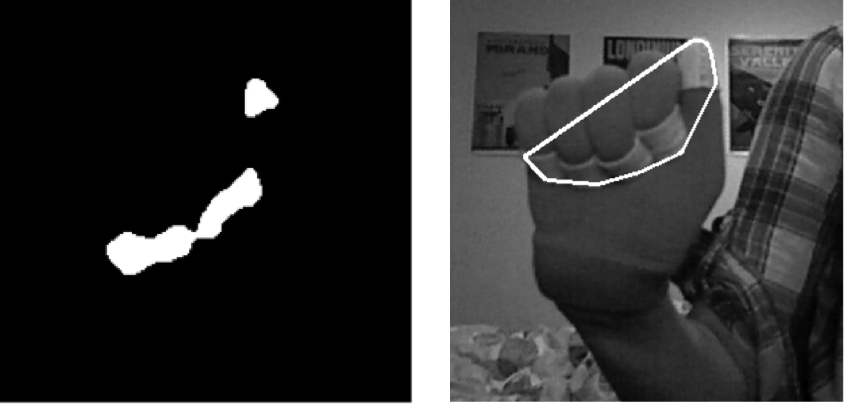
\includegraphics[scale=0.7]{Hull.png}
  \caption{Convex Hull}
  \label{hull}
\end{figure}

We can convert this shape into a feature vector using shape descriptors. The central image moments are perhaps the simplest image descriptors; they describe the distribution of a shape about its x and y axes. Each raw moment, \(M_{pq}\), is defined as follows:
\begin{equation*}
M_{pq} = \int_{-\infty}^\infty \int_{-\infty}^\infty x^p y^q f(x,y) dxdy
\end{equation*}
We use the central normalized moments, \(n_{pq}\), which have been normalized and repositioned about the centroid, making them both shift- and scale-invariant. This is a necessary feature of all our image descriptors; recognition of the sign should be independent of the hand’s position in the frame,or distance from the Kinect. When classifying signs we use the first seven central moments. (ie. \(p + q  <= 3\) )

\paragraph{Classification}
For our initial prototype, we chose to use a support vector machine (SVM) classifier. This was intended to be an intermediate classifier used to demonstrate the efficacy of our preprocessing and feature selection techniques in distinghuising hand posture. More advanced classifiers would later be implemented to recognize signs involving motion. As such, SVM was chosen mainly because the developers are already familiar with training support vectors machines, and they are widely used in industry including in our literature review. At this point, 

Every labelled sample in our training library has a single feature vector of length n associated with it; these can be viewed as points within an n-dimensional feature space. During training, the support vector machine constructs a series of hyperplanes to separate points belonging to different classes; this plane serves as the class boundary when predicting future samples. The goal of the SVM is to maximize the margin between the boundary and the nearest points on either side while minimizing the number of misclassifications. These points can also be transformed into a higher-dimensional feature space to obtain a more flexible boundary. A simple parameter grid search was used to optimize the classifier.

\subsubsection{Prototype \#2}
Beginning in January, we shifted focus towards classification of dynamic signs. This necessitated changes to the feature extraction and classification components of the system to accommodate the added temporal information. The video preprocessing steps and calculation of the hull features remained largely unchanged, having demonstrated their efficacy in the static classifier. An intermediate prototype implementing a working dynamic sign classifier was presented at the Open House on February 4th; this prototype was capable of recognizing  vocabulary signs but required some intervention from the demonstrators in order to determine colour thresholds and gesture start and end points. To simplify both classification and data collection, we chose a set of ten vocabulary signs to train our classifier. A description of the selected signs can be found in Appendix A.  

\paragraph{Feature Extraction}
The feature set for the dynamic classifier is expanded from the original prototype, in order to include the position and posture of both hands. One complete feature vector is calculated for each video frame, so that the input to the classifier is a timeseries matrix of \(n\) features by \(t\) frames.

Based on the performance of the static classifier, the central moments of the hull are capable of distinguishing between various hand postures, so filtering and calculation for these features is the same as the previous prototype. The same features are replicated for the left hand by detecting the red markers on the second glove. 

In addition, the new feature vector includes the centroids of both hands, allowing us to classify a sign based on overall motion. The shape of each hand is found by detecting blue regions adjacent to the coloured finger markers, and the centroid is calculated from the combined shape. Initially a 3-dimensional position was taken, using the Kinect’s depth camera; but the depth dimension was later removed as it did not add skill to the classifier. All position features are renormalized over the range 0 to 1. To further reduce noise, the entire timeseries is smoothing by taking the average of the last five feature vectors.

\begin{figure}[h!]
  \centering
  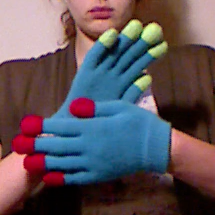
\includegraphics[scale=.7]{fe1.png}
  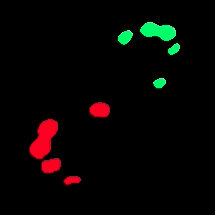
\includegraphics[scale=.7]{fe2.png}
  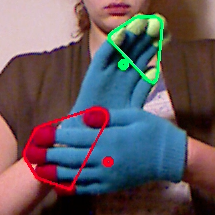
\includegraphics[scale=.7]{fe3.png}
  \caption{Feature Extraction Steps}
  \label{fe_steps}
\end{figure}

\paragraph{Classification}
The support vector machine used in the previous prototype is not well suited to classifying features collected over time. After considering several options, we chose to use Hidden Markov Models as our dynamic classifier. A Hidden Markov Model represents a process as a series of connected states; for each connection between states there is some constant probability that a process currently in the first state will move into the second during the next time step. These transition probabilities are defined in the matrix \(A\), where:
\begin{equation*}
  a_{ij} = P[q_{t+1} = \text{State}_j | q_t = \text{State}_i], \:\: 1 \leq i,j \leq N
\end{equation*}
There is also a vector, \(\lambda\), that gives the probability of starting the process in a given state.
\begin{equation*}
  \lambda_{i} = P[q_0 = \text{State}_i], \:\: 1 \leq i \leq N
\end{equation*}

While the states themselves are unobserved, or hidden, each state is associated with possible observations. The set \(B\) describes the relationship between states and observations; each element \(b_j(k)\) gives the probability of recording observation \(k\) while the model is in state \(j\). 
\begin{equation*}
  b_j(k) = P[\text{Obs}(k)| q_t = \text{State}_i], \:\: 1 \leq j \leq N
\end{equation*}

The element \(b_j(k)\) can either be a continuous probability distribution or a discrete set of probabilities. In our case, the observations are the features extracted from the processed video and \(b_j(k)\) is a continuous distribution approximated using a Gaussian Mixture Model.

Given a complete Hidden Markov Model, we can estimate the likelihood that a new set of observations could have been generated by the given model, using a Forward-Backward Procedure. Given this capability, we can classify features by creating a Hidden Markov Model for each of the candidate signs and selecting the model that has the highest probability of generating the given feature set. 

To create the models, the probabilities \(A\), \(B\) and \(\lambda\) are estimated based on existing observations by using a Viterbi algorithm. Over the course of the term, we recorded a series of labelled Kinect data samples using the fakenect utility; each sample consists of a subject performing one of the ten selected signs while wearing the gloves. The final dataset consisted of 22 samples for each sign, performed by 8 different users.  

The other model parameters, namely the number of states, are chosen by randomly generating sets of parameters and training models for each. The classifier with the best performance is selected for use in the prototype.

\paragraph{User Interface}
An initial user interface was developed for use at the Open House demonstration. This demo prompted the user to perform a specific sign, recorded video from the Kinect until it was stopped and then displayed a congratulatory message if the sign was classified correctly. 

This version of the prototype required significant human intervention in order to function. Most notably, the system required user input to start and stop the Kinect recording; as the user was sitting back from the screen and wearing gloves, this was usually done by the person directing the demonstration. Furthermore, the system had to be pre-calibrated prior to the demonstration and then re-calibrated every time the lighting changed significantly. Several improvements were made in the subsequent prototype that automated these inputs. 

\subsubsection{Prototype \#3}
The final prototype included several major improvements to the basic classification system presented at the Open House. These include the implementation of a continuous, rather than isolated, sign recognition system, the addition of automatic calibration, and a more polished user interface. 

\paragraph{Continuous Recognition}
In the previous prototype, the samples used for training and classification lasted only for the duration of the gesture; we refer to this as isolated recognition. Continuous recognition, by contrast, involves detecting and classifying gestures within a video sample as it plays and ignoring segments that do not contain a gesture; a process known as gesture spotting. We require a method to produce candidate timeseries for classification and a method to determine whether a candidate timeseries contains contains a gesture or not; we use a sliding window method and a threshold model to solve these problems respectively. 

The threshold model used in the final prototype was first proposed by Lee and Kim\cite{LeeKim}. Ideally, we would like to accept a detected sign only if the gesture model has a high enough likelihood, the same metric used to choose the best-fitting model. Unfortunately, the likelihood seems to work only as a relative metric, and performs poorly when compared with an absolute threshold. So instead, we create a threshold model composed of the states of all ten sign models. In this new model, the observations and the self-transition probabilities are preserved, but the there is always an equal probability of moving to any other state in the network. The result is an extremely weak model capable of matching any gesture; however, the original models will do a better job of describing their respective gestures, because they better capture the transition probabilities. Therefore, the likelihood from the new model can be used as an adaptive threshold; if the sign model scores higher than the threshold model, the sign is accepted. 

We use a sliding window approach to produce finite inputs to the Hidden Markov Model classifier. At each frame we define a window of no more than 100 preceding frames. If no sign is detected in this window, the window is progressively shortened until either a sign is found or the number of frames falls below a predefined minimum. After a sign is found, the window will reset itself to zero frames when the system no longer detects that sign being performed.

With the addition of an adaptive threshold, we can also perform simple yes-no classification as well as multi-class classification. In the final prototype, only the subset of signs expected by the activity are evaluated against the threshold, further reducing the misclassification rate.

\paragraph{Automatic Calibration}
We developed an automated calibration process for inclusion in the demo. This process was designed to recognize a static position with both hands open and facing the camera.  The user holds their gloved hands out in front of the camera and a minimization algorithm searches for the optimal thresholds within the colour space based on the Euclidean distance between the current and expected hull features. The algorithm uses a random walk with occasional random restarts, preserving the best performing thresholds. Calibration stops when it detects five fingers on each hand and the feature error is below some threshold for at least 10 consecutive frames. In good lighting, this process takes no more than a minute.

\paragraph{User Interface}
Two separate interfaces were developed for the final prototype, demonstrating both single- and multi-class classification. Both took the form of simple games in which the user was prompted to perform either a single sign or a choice of signs. Upon recognizing a gesture, the system would respond appropriately. No other user action was required during the game.

The first interface was a simple vocabulary game, similar to the previous prototype. The user would be given the name a sign and the system would display a congratulatory message upon recognizing it. 

The second interface was a game entitled “Would You Rather?”  Users were posed a multiple-choice question such as “Would you prefer a BIG dog or a SMALL dog?” and had to perform the appropriate sign to indicate their choice. Upon detecting a sign, the system would respond with a comment, occasionally humorously. This second game was meant to demonstrate the possibility of using the system for more natural interactions rather than simple language exercises, allowing the user to develop conversational skills.

\subsection{Notable Technical Challenges and Resolutions}
\subsubsection{Decision to Use Coloured Markers}
Both bare hand tracking and tracking using artificial markers were considered as methods to detect the user’s hand and fingers in the video stream.

\begin{table}[h]
\centering
\caption{Hand-Tracking Libraries}
\label{libraries}
\begin{tabular}{|p{5cm}| p{11cm} |}
\hline
\textbf{Name/Company}                                                                      & \textbf{Capabilities}                                                                                                                                \\ \hline
3D Hand Tracking, The Foundation for Research and Technology-Hellas (FORTH) \cite{FORTH} & Creates a model of the hand that is capable of tracking individual fingers without losing them when out of site. Advertises no calibration required. \\ \hline
TuioKinect hand tracker for Kinect \cite{tuiokinect}                                     & Can recognize large hand gestures but does not have individual finger recognition.                                                                   \\ \hline
Hand Kinetics \cite{handkinetics}                                                        & Hand and segment model created with classifiers appears to capture fingers very well. Not yet commercially available.                                \\ \hline
\end{tabular}
\end{table}

The hand-tracking libraries in Table \ref{libraries} were investigated. These libraries are intended to identify a user’s bare hand. It was determined that none of these libraries was viable for this project. The Hand Kinetics application is not yet commercially available. The TuioKinect hand tracker does not support finger recognition and therefore not capable of collecting sufficient data to create an accurate classifier. The library by FORTH could not reliably track a hand as demonstrated in Figure \ref{forth}. 

\begin{figure}[h!]
  \centering
  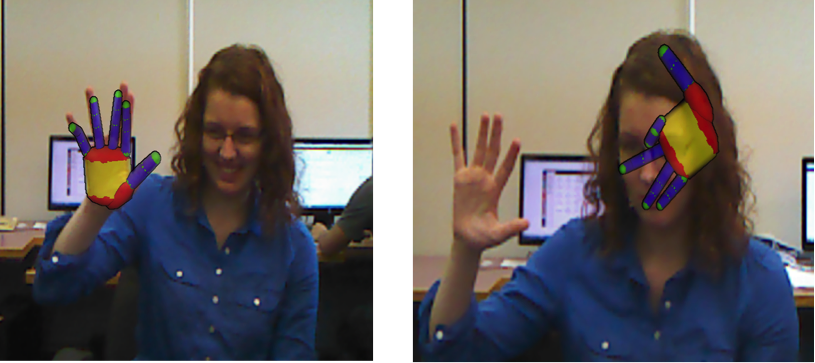
\includegraphics[scale=0.8]{FORTH.png}
  \caption{Example of an Existing Hand-Tracking LIbrary}
  \label{forth}
\end{figure}

The difficulty in tracking a bare hand is due to several factors. First, skin colour differs widely between people. When a person’s face is also in the frame, an algorithm may be unable to differentiate between the facial skin and the skin of the hand. It is also difficult to identify fingers and fingertips from the rest of the hand, specifically when a user’s fingers overlap the palm, such as in the ASL sign for the letter ‘A’. 

The use of a glove solves the problem of differentiating skin colours, and allows the application of artificial markers to identify specific regions of the hand such as the fingertips or palm. In the realm of a teaching application, requiring a user to wear a glove is reasonable provided the glove does not inhibit the user’s motion and does not impose a significant increase in cost.

\subsubsection{Choosing a Classification Framework}
Several alternatives were considered before we decided to use Hidden Markov Models as a dynamic classifier. Examples include Fourier features, Discrete Cosine Transform, Discrete Wavelet Transform, Dynamic Time Warping, Compression-Based Dissimilarity and Time Series Clustering. Broadly speaking, these techniques fall into one of two categories: they either transform a timeseries into a new feature space with fewer dimensions, or they define a similarity metric between different timeseries’ to be used in a Euclidean distance or Nearest Neighbour classifier. Most of these, therefore, make some assumptions about what aspects of the input signal are important; for example, the fundamental frequencies (Discrete Cosine Transform) or a particular pattern of peaks and valleys (Dynamic Time Warping). Based on the variation in cadence and expression that is available to users when signing, we do not believe that any of these methods would be well-suited to classifying ASL.

Hidden Markov Models are widely used in the literature, particularly in gesture recognition. Rather than trying to transform or simplify a timeseries before passing it into a classifier, which requires a greater degree of domain knowledge about the input signal, a Hidden Markov Model is designed to learn the temporal patterns of a process and associated observations based on training data. Furthermore, this method of classification is far more intuitive; there is a meaningful mapping between the sign model and the motions being performed. This has potential benefits when debugging the models or giving feedback to the user. 

\subsubsection{Lighting Calibration}
It became apparent early in the design process that the colour detection system was fairly sensitive to lighting. Changes in environmental lighting required that we determine optimal thresholds for the colour filters every time the kinect moved to a new location. In the beginning, we developed a tool to estimate the thresholds by having a user indicate the regions of the the video frame that were the appropriate colour. This solution was clearly not adequate for a final prototype as it required too much expert input from the user.

We considered having the user align their hand with a hand on the screen, but we were eventually inspired by our original static classifier prototype; the feature vector we use to distinguish hand shapes can also be used to determine how well a colour filter can match an expected output. This approach requires only a fairly natural interaction on the part of the user.

The error is defined as the Euclidean distance between the current central moments of the convex hull detected by the filter and those of an ideal shape. We found that this error function was not continuous enough for techniques like gradient descent, so we minimize the error by taking a random walk through the colour space with occasional random restarts, and record the best thresholds. We also found that the hull shape was too general and the minimization would sometimes converge on noise patterns that produced a similar shape. We prevent this by adding the requirement that the camera must detect exactly five fingers and pass the error threshold for ten consecutive frames.

\newpage
\section{Design Testing and Validation}
Two separate tests exist to validate the Hidden Markov Model classifier; one for isolated recognition, in which the endpoints of the observation vector are predefined, and continuous recognition, which makes use of the threshold model and validates against a continuous stream of video. 
\subsection{Isolated Recognition}
Isolated recognition testing is performed as the models are trained. The training library is split into five sections, or folds, and the classifier is trained using only four of the five folds. The resulting classifier is used to classify the samples in the remaining fold and the results are recorded. This is repeated with a different fold left out of training until each sample in the dataset has been classified once. This process, called cross-validation, is usually performed multiple times with varying parameters; the set of parameters with the best cross-validation accuracy is used to train a classifier using the entire training set. In addition to accuracy, this test produces a confusion matrix, indicating which types of misclassifications are common.

Because this test is an automated part of the training process, it is often used to compare the performance of models and data generated using different techniques. For example, isolated recognition performance was used to determine the best way to calculate the hand centroids and the amount of temporal smoothing to use.

\subsubsection{Results}
Table \ref{isolated} shows the isolated recognition confusion matrix for the classifier used in the final prototype. To understand the confusion matrix, elements on the diagonal are correct classificatio, or "True Positives," and all other elements are misclassifications. We can use the confusion matrix to investigate common mistakes made by the model; in this case, for example, MOTHER is often confused with CAT. The overall accuracy of the classifier is the number of true positives over the total number of samples. The isolated recognition accuracy of this model is about 76\%.

\begin{table}[h]
\centering
\caption{Isolated Recognition Results}
\label{isolated}
\begin{tabular}{ll|c|c|c|c|c|c|c|c|c|c|}
\cline{3-12}
                               &                                  & \multicolumn{10}{|c|}{Actual}                                                    \\ \cline{3-12} 
                               &                                  & \rotatebox[origin=c]{90}{BIG} & \rotatebox[origin=c]{90}{CAT} & \rotatebox[origin=c]{90}{  FAVOURITE  } & \rotatebox[origin=c]{90}{HOUSE} & \rotatebox[origin=c]{90}{MORE} & \rotatebox[origin=c]{90}{MOTHER} & \rotatebox[origin=c]{90}{MOVIE} & \rotatebox[origin=c]{90}{RED} & \rotatebox[origin=c]{90}{SMALL} & \rotatebox[origin=c]{90}{  SWEETHEART  } \\ \hline
\multicolumn{1}{|c}{}          & \multicolumn{1}{|l|}{BIG}        & 16  & 0   & 2         & 2     & 1    & 1      & 2     & 0   & 1     & 2          \\ \cline{2-12} 
\multicolumn{1}{|l}{}          & \multicolumn{1}{|l|}{CAT}        & 0   & 13  & 0         & 0     & 0    & 7      & 0     & 0   & 0     & 0          \\ \cline{2-12} 
\multicolumn{1}{|l}{}          & \multicolumn{1}{|l|}{FAVOURITE}  & 0   & 2   & 20        & 0     & 0    & 0      & 0     & 0   & 0     & 0          \\ \cline{2-12} 
\multicolumn{1}{|l}{}          & \multicolumn{1}{|l|}{HOUSE}      & 5   & 0   & 0         & 19    & 2    & 0      & 0     & 0   & 0     & 0          \\ \cline{2-12} 
\multicolumn{1}{|l}{Predicted} & \multicolumn{1}{|l|}{MORE}       & 0   & 0   & 0         & 0     & 15   & 0      & 0     & 0   & 0     & 0          \\ \cline{2-12} 
\multicolumn{1}{|l}{}          & \multicolumn{1}{|l|}{MOTHER}     & 1   & 5   & 0         & 1     & 0    & 11     & 0     & 1   & 0     & 0          \\ \cline{2-12} 
\multicolumn{1}{|l}{}          & \multicolumn{1}{|l|}{MOVIE}      & 2   & 0   & 0         & 0     & 1    & 0      & 16    & 0   & 0     & 0          \\ \cline{2-12} 
\multicolumn{1}{|l}{}          & \multicolumn{1}{|l|}{RED}        & 0   & 2   & 0         & 0     & 0    & 2      & 0     & 20  & 0     & 0          \\ \cline{2-12} 
\multicolumn{1}{|l}{}          & \multicolumn{1}{|l|}{SMALL}      & 0   & 0   & 0         & 0     & 3    & 1      & 0     & 0   & 19    & 0          \\ \cline{2-12} 
\multicolumn{1}{|l}{}          & \multicolumn{1}{|l|}{SWEETHEART} & 0   & 0   & 0         & 0     & 0    & 0      & 3     & 1   & 0     & 19         \\ \hline
\end{tabular}
\end{table}

\subsection{Continuous Recognition}
In the continuous recognition test, one tester sits in front of the Kinect and signs each of the candidate signs five times. Another tester records correct classifications, misclassifications, and false positives into a confusion matrix similar to the one used for isolated recognition. If two classifiers are being compared, they must be tested in back-to-back sessions using identical calibration and lighting.

Despite its similarity to the previous test, continuous recognition testing is important to understand the error introduced by the threshold model and give a more realistic estimate of performance. Because the test is currently performed manually, it is not typically used to motivate decisions. However, the results of this test represent the most realistic benchmark for the system’s accuracy. In the future, we recommend more extensive continuous testing be performed.

\subsubsection{Results}
Table \ref{continue} shows the continuous recognition confusion matrix for the classifier used in the final prototype. This matrix is similar to the one used for isolated recognition, but with two additional categories. "Not Recognized" refers to the case where a sign is performed at the system gives no response. "False Positive" refers to the opposite case where the system makes a classification when no sign has been performed. The continuous recognition accuracy of this classifier is 60\%.  

\begin{table}[h]
\centering
\caption{Continuous Recognition Results}
\label{continue}
\begin{tabular}{ll|c|c|c|c|c|c|c|c|c|c|c|c|}
\cline{3-14}
                               &                                  & \multicolumn{12}{c|}{Actual}                                                    \\ \cline{3-14} 
                               &                                  & \rotatebox[origin=c]{90}{BIG} & \rotatebox[origin=c]{90}{CAT} & \rotatebox[origin=c]{90}{  FAVOURITE  } & \rotatebox[origin=c]{90}{HOUSE} & \rotatebox[origin=c]{90}{MORE} & \rotatebox[origin=c]{90}{MOTHER} & \rotatebox[origin=c]{90}{MOVIE} & \rotatebox[origin=c]{90}{RED} & \rotatebox[origin=c]{90}{SMALL} & \rotatebox[origin=c]{90}{  SWEETHEART  } & \rotatebox[origin=c]{90}{  Not Recognized  } & \rotatebox[origin=c]{90}{  False Positive  }\\ \hline
\multicolumn{1}{|c}{}          & \multicolumn{1}{|l|}{BIG}        & 5  & 0   & 0         & 0     & 0    & 0      & 0     & 0   & 0     & 0   &0&0       \\ \cline{2-14} 
\multicolumn{1}{|l}{}          & \multicolumn{1}{|l|}{CAT}        & 0   & 5  & 0         & 0     & 0    & 0      & 0     & 0   & 0     & 0   &0&0       \\ \cline{2-14} 
\multicolumn{1}{|l}{}          & \multicolumn{1}{|l|}{FAVOURITE}  & 0   & 0   & 4        & 0     & 0    & 0      & 0     & 0   & 0     & 0   &1&2       \\ \cline{2-14} 
\multicolumn{1}{|l}{}          & \multicolumn{1}{|l|}{HOUSE}      & 1   & 0   & 0         & 0    & 0    & 0      & 0     & 0   & 0     & 0   &4&0       \\ \cline{2-14} 
\multicolumn{1}{|l}{Predicted} & \multicolumn{1}{|l|}{MORE}       & 0   & 0   & 0         & 0     & 3   & 0      & 0     & 0   & 1     & 0   &1&0       \\ \cline{2-14} 
\multicolumn{1}{|l}{}          & \multicolumn{1}{|l|}{MOTHER}     & 0   & 2   & 0         & 0     & 0    & 0     & 0     & 0   & 0     & 0   &3&0       \\ \cline{2-14} 
\multicolumn{1}{|l}{}          & \multicolumn{1}{|l|}{MOVIE}      & 0   & 0   & 0         & 0     & 0    & 0      & 5    & 0   & 0     & 0   &0&0       \\ \cline{2-14} 
\multicolumn{1}{|l}{}          & \multicolumn{1}{|l|}{RED}        & 0   & 0   & 0         & 0     & 0    & 0      & 0     & 0  & 0     & 0   &5&3       \\ \cline{2-14} 
\multicolumn{1}{|l}{}          & \multicolumn{1}{|l|}{SMALL}      & 0   & 0   & 0         & 0     & 0    & 0      & 0     & 0   & 4    & 0   &1&0       \\ \cline{2-14} 
\multicolumn{1}{|l}{}          & \multicolumn{1}{|l|}{SWEETHEART} & 1   & 0   & 0         & 0     & 0    & 0      & 0     & 0   & 0     & 4  &0&0       \\ \hline
\end{tabular}
\\
\begin{tabular}{l c}

\textbf{True Positives} & 30 \\
\textbf{Misclassifications} & 5 \\
\textbf{Not Recognized} & 15 \\
\textbf{False Positives} & 5 \\

\end{tabular}

\end{table}

\subsection{Lighting Tests}
All ten signs were tested in 3 lighting conditions for performance: natural light, a single lamp, and ambient artificial lighting. Each sign was performed five times during one test. Lighting scenarios were tested twice. The sign was only counted as “recognized” if it passed the threshold model for the correct sign. A false positive is the apparent recognition of a sign when none is being performed. 

A fourth lighting condition was considered, in which a single light source was located behind the user, but this rendered the user very dark and the colours of the glove were indistinguishable either through manual or automated calibration.

\subsubsection{Results}
Table \ref{light} gives a summary of the results of testing the system in different lighting conditions. Complete results can be found in Appendix B.

\begin{table}[h]
\centering
\caption{Summarized Lighting Test Results}
\label{light}
\begin{tabular}{|l|c|c|c|}

\hline
 & \textbf{Natural} & \textbf{Lamp} & \textbf{Ambient} \\ \hline
\textbf{True Positives} & 46\% & 56 \% & 70\% \\ \hline
\textbf{Misclassifications} & 11\% & 15\% & 6\% \\ \hline
\textbf{Not Recognized} & 43\% & 39\% & 24\% \\ \hline
\textbf{False Positives} & 0 & 0 & 0 \\ \hline

\end{tabular}

\end{table}

Natural light provided the least number of true positives. Checking the calibration after the test showed that the lighting conditions had varied slightly, causing the red thresholds to no longer be accurate. 

A single lamp proved to achieve a higher number of true positives and fewer “not recognized” signs than natural light, but it also misclassified more signs. Misclassifications are less likely to be a result of lighting and more likely to be related to the specific features and the mechanics of the classifier. Ambient light proved the most reliable, with the highest number of true positives and few misclassifications. No false positives were recorded during any tests.

\subsection{Discussion}

\subsubsection{Model Validation}
Perhaps the most notable result from the model validation tests is the difference in performance between the isolated and continuous recognition tests. Performance in isolated recognition almost meets our original requirement of 80\% accuracy but the continuous case performs significantly worse. 

The largest source of error in continuous recognition is the system failing to recognize the sign, indicating that the threshold model may be too strict. Finding ways to relax the threshold model may mitigate this, but it may also increase the rate of misclassifications and false positives. The model must be designed with this tradeoff in mind; in a teaching application, it is probably better to have the user perform the sign again than to give incorrect feedback.
In addition, the isolated recognition test has a slight advantage in that it the test and training data come from the same library. Samples are often recorded consecutively with no change in position or lighting, so there may be a lot of consistency between samples. By contrast, the continuous test is always performed manually and the classifier is required to generalize to a new environment. This may contribute to a loss in skill that would be improved by greater robustness to lighting.

Unfortunately, the continuous recognition accuracy is more representative of the expected performance. This accuracy fails to meets our requirements and a significant amount of work is required to improve performance. However, the isolated recognition performance indicates that there is indeed room for improvement.

\subsubsection{Robustness to Lighting}
Based on our testing, the system works well for common indoor lighting conditions, but starts to lose skill when natural or focused light is introduced. We have found that the system does not respond well to changing light or different light levels within the frame. More problematic are the cases where the system cannot be calibrated, such as the common case of a light source behind the user. While it is reasonable to expect that this system will mainly be used indoors in moderate lighting, such limitation and losses in skill will be frustrating for the user. The system does not yet meet our requirements for robustness to lighting but we believe the current performance represents a good basis for improvement. 

\newpage
\section{Recommended Design Modifications}
\subsection{Robustness to Lighting}
As demonstrated during testing, lighting has huge impact on performance; the system performs well only in certain environments and only if the lighting is static. The current system is reliable after calibration, provided the ambient lighting conditions do not change. Should this happen, extracted features become inaccurate and the performace of the system suffers. Techniques such as adaptive colour thresholding could solve this problem by dynamically altering the thresholds for the colours of interest. Some algorithms already exists, such as one created by Deshmukh and Shinde \cite{adaptiveSegmentation} that implements artificial neural networks to vary thresholds based on the saturation and intensity of the image in question. Improving the robustness to lighting will have a measurable impact on accuracy and should be made a top priority.

\subsection{Improved Classification}
Classification accuracy should be improved before considering any commercial applications of this system. At present it is not entirely clear what will affect the accuracy aside from improving the robustness to lighting. We can only recommend additional experiments. Additional features, such as velocity or the silhouette of the entire hand, or modifications to existing features could conceivably improve the performance. Likewise, there may be other classification frameworks more suited to this task.

We might also experiment with finding the optimal model parameters. In the case of Hidden Markov Models, the main parameter to be chosen is the number of hidden states in each model. These parameters are currently chosen randomly and seem to contribute little to performance. (ie. we have yet to discover any relationships between number of states and skill) Often the number of states is chosen by hand based on the properties of the gesture, but this requires a degree of expertise and it not feasible for larger libraries. Some heuristic algorithms exist to optimize the internal structure of HMMs including hill-climbing\cite{opto1} and genetic algorithms\cite{opto2}; experiments with these might have an effect on the classifier performance.

Finally, as the continuous recognition test represents a more measure of statistic performance, this test should be automated and performed every tim the model is trained. This might be done by recording longer samples with multiple signs and labelling the times at which signs occur. Decisions regarding the optimal models should be made based on this test rather than on isolated recognition.

\subsection{Improved User Interface}
As previously mentioned, a comprehensive user interface was not included in the scope of this project. However, a pleasant, fun, and user-friendly interface would have great impact on the user’s experience with the system. Should this project be brought to a commercial level, a full user interface is required. In particular, the goal of such an interface should be to engage the user and encourage them to develop conversational skills, such as constructing full sentences and responding to in-game characters, rather than rote memorization. Additional research into language learning should inform the design of the interface.

To help improve the interface, it is recommended that future iterations provide the user with more detailed feedback. A possible modification would be to evaluate the score of a user’s attempt based on its proximity to the threshold value. It would be useful for the user to know what he or she has done wrong, in addition to the fact that the sign was incorrectly performed. This could potentially be indicated through highlighting the differences between the user’s attempt and a video of a properly executed sign.

\subsection{Gloves and Camera}
Some users found the gloves to be too small for their hands. The current glove prototype is made of extremely cheap materials, and so it is recommended that more durable materials be implemented in the future to create gloves in multiple sizes. 

Alternatively, if fingertips could be detected reliably on bare hands it may become possible to achieve similar results without gloves. Microsoft will be releasing the Kinect for Windows V2 summer 2014 \cite{kinect2}, and boasts higher precision and improved skeletal tracking \cite{kinect2capabilities}. Some fingertip tracking already exists, using the Kinect V1 and OpenNI \cite{fingertips}, and so it can be projected that with an improved sensor this tracking may become sufficiently reliable. Implementing this may require some changes to the feature space.

On the other hand, since the depth feature was removed from classification, the current prototype uses no information from the Kinect that could not be provided by any other camera. Using a generic camera would make the system far more accessible to users as webcams are widely used and much less expensive than the Kinect. Market research would determine whether it is better to work towards detection without gloves by using more advanced sensors or keep the gloves in favour of using more available hardware.

\subsection{Scaling Up}
While we believe that classifying ten signs is sufficient to demmonstrate feasibility, it is insufficient for any practical teaching application. Attempting to expand the library to include a beginner's vocabulary will introduce some new challenges. Classification accuracy, data collection and speed will be negatively impacted.

Additional features may be necessary in order to capture a larger set of signs. Potential new features include the location of the users’ eyes or face, since some signs take meaning from the location of the hands with respect to the user’s head. For instance, the sign MOTHER is exactly the same as the sign FATHER, except that the former is located at the chin and the latter at the forehead.

Currently, data collection is a long and tedious process and is not suitable for the creation of a large-scale sign database. We recommend that the data collection become part of the system as a Game With a Purpose, a human computation technique developed by Luis von Ahm that collects data through human-computer interaction. We propose that a user be asked to perform certain signs that do not yet have a model, and then be asked to name or judge other users’ attempts. Only samples that have been judged positively by multiple users would then be used to create a sign model. These tasks can be integrated into the interface as educational activities; for example, asking the user to copy an on-screen avatar for practice. The concept of a Game With a Purpose is powerful because it can used to accomplsih multiple objectives. In addition to automating the data collection process, these methods could also foster a sense of community in the userbase through communication with other sign language learners and contribution to the system. 


\newpage
\section{Timeline and Project Management}
\subsection{Timeline}
The Gantt chart (Figure \ref{gantt}) summarizes the use of time throughout the project. This chart very closely resembles previous charts, as the project remained on track for its entirety. Many activities overlapped, and team members often worked on separate tasks when possible. 
 
\begin{figure}[h!]
  \centering
  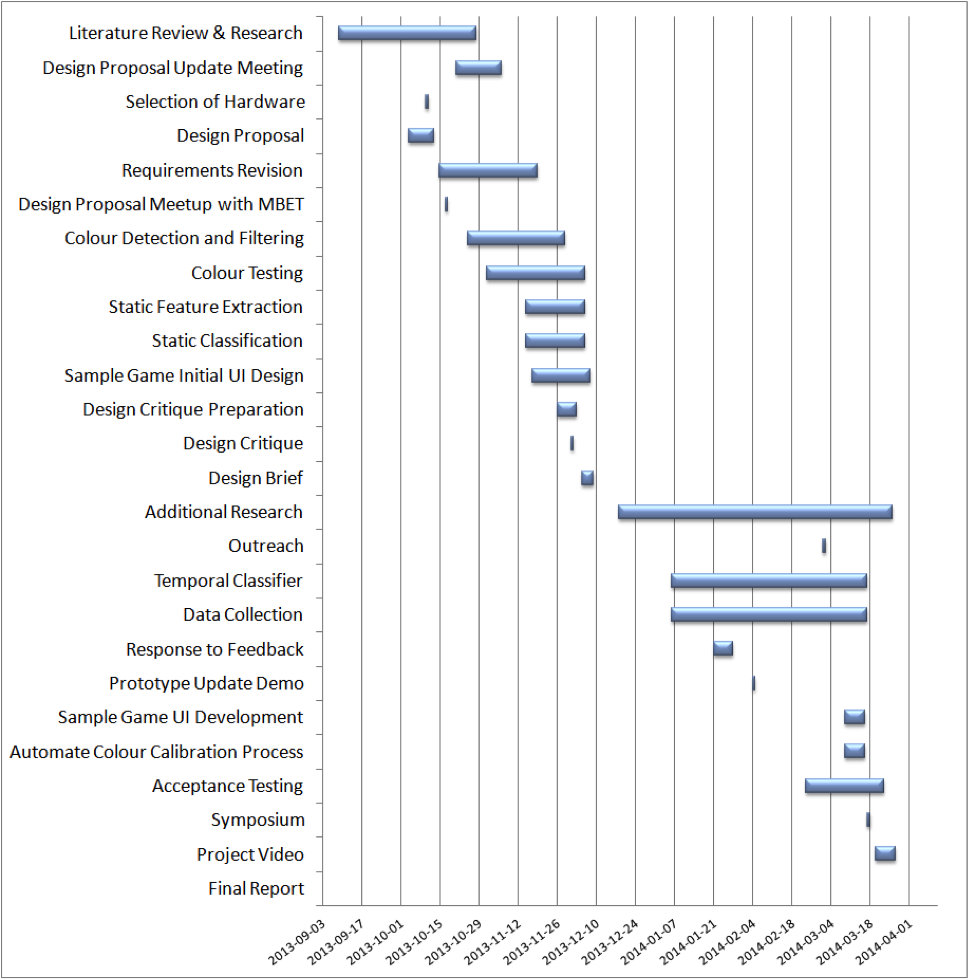
\includegraphics[scale=0.8]{Gantt.png}
  \caption{Gantt Chart}
  \label{gantt}
\end{figure}

\subsection{Member Contributions}

During the Fall 2013 term, Sara was responsible for colour analysis and testing, glove design, user interface mockups,meeting minutes, communication with supervisors, and the research ethics approval application. Jennifer was responsible for leading the literature review and the development and testing of the initial feature extraction and classification techniques.
Jennifer and Sara collaborated on the preparation of the Dragon’s Den demo, and much of the
decision making was shared.

During the Winter 2014 term, Sara continued to be the lead communications group member and recorded meeting minutes. She collected the bulk of user data that allowed for the creation of the model. She did initial research into automatic calibration methods, and conducted lighting tests. She was responsible for the project poster and video, and created the user interface for symposium. Jennifer led the development, training and validation of the sign classifier. She was also responsible for continued research efforts and improvements to feature extraction.

\subsection{Document Management}
Meeting minutes, brainstorming and progress are stored in a shared Google Drive folder. This folder serves as a digital notebook for both group members. A repository on GitHub is used for project code and version control. Because the Kinect video data used to create a classification
model is so large, a subscription Dropbox folder stores this data as a backup to the data stored on an external hard drive.

\subsection{Group and Supervisor Meetings}
The group met with the supervisors once a week, for 15-30 minutes. Group members met officially 1-2 times a week, but updates and discussion occurred frequently and organically due to living in the same residence. This system was effective.

\subsection{Financial Budget}
Hardware (personal computers and Kinect camera) were possessed by group members prior to the project and are therefore not included in the budget. Likewise, software libraries are all open source and have no financial cost. The financial budget is allocated towards glove materials and a monthly dropbox fee, used for sharing the large training library between group members.

\begin{table}[h]
\centering
\caption{Budget}
\label{budget}
\begin{tabular}{|l|c|}

\hline
\textbf{Item} &     \textbf{Cost} \\ \hline
Glove Materials (Several Iterations)  &   \$30.00 \\ \hline
Dropbox subscription for additional space, \$10/month for 6 months  &  \$ 60.00 \\ \hline
\textbf{Total} &   \$90.00 \\ \hline
\end{tabular}

\end{table}

\newpage
\section{Conclusion}
The final prototype is capable of recognizing 10 trained signs with reasonable accuracy in most indoor ambient lighting environments. Additional work is required in almost every aspect of the system; notable weaknesses include poor robustness to lighting conditions as well as reduced performance in continuous recognition. Nevertheless, we believe this prototype shows the potential for the application of computer vision and classification techniques in an American Sign Language teaching tool. In particular, we have shown that the hard problem of real-time translation can be made tractable in pedagogical applications using simplifying techniques such as coloured markers. We believe this project has potential and should be developed further.


\newpage
\onehalfspacing

\bibliographystyle{IEEEtran}
\bibliography{fydp}


\newpage
\tocsection{Appendix A - Selected Signs}
  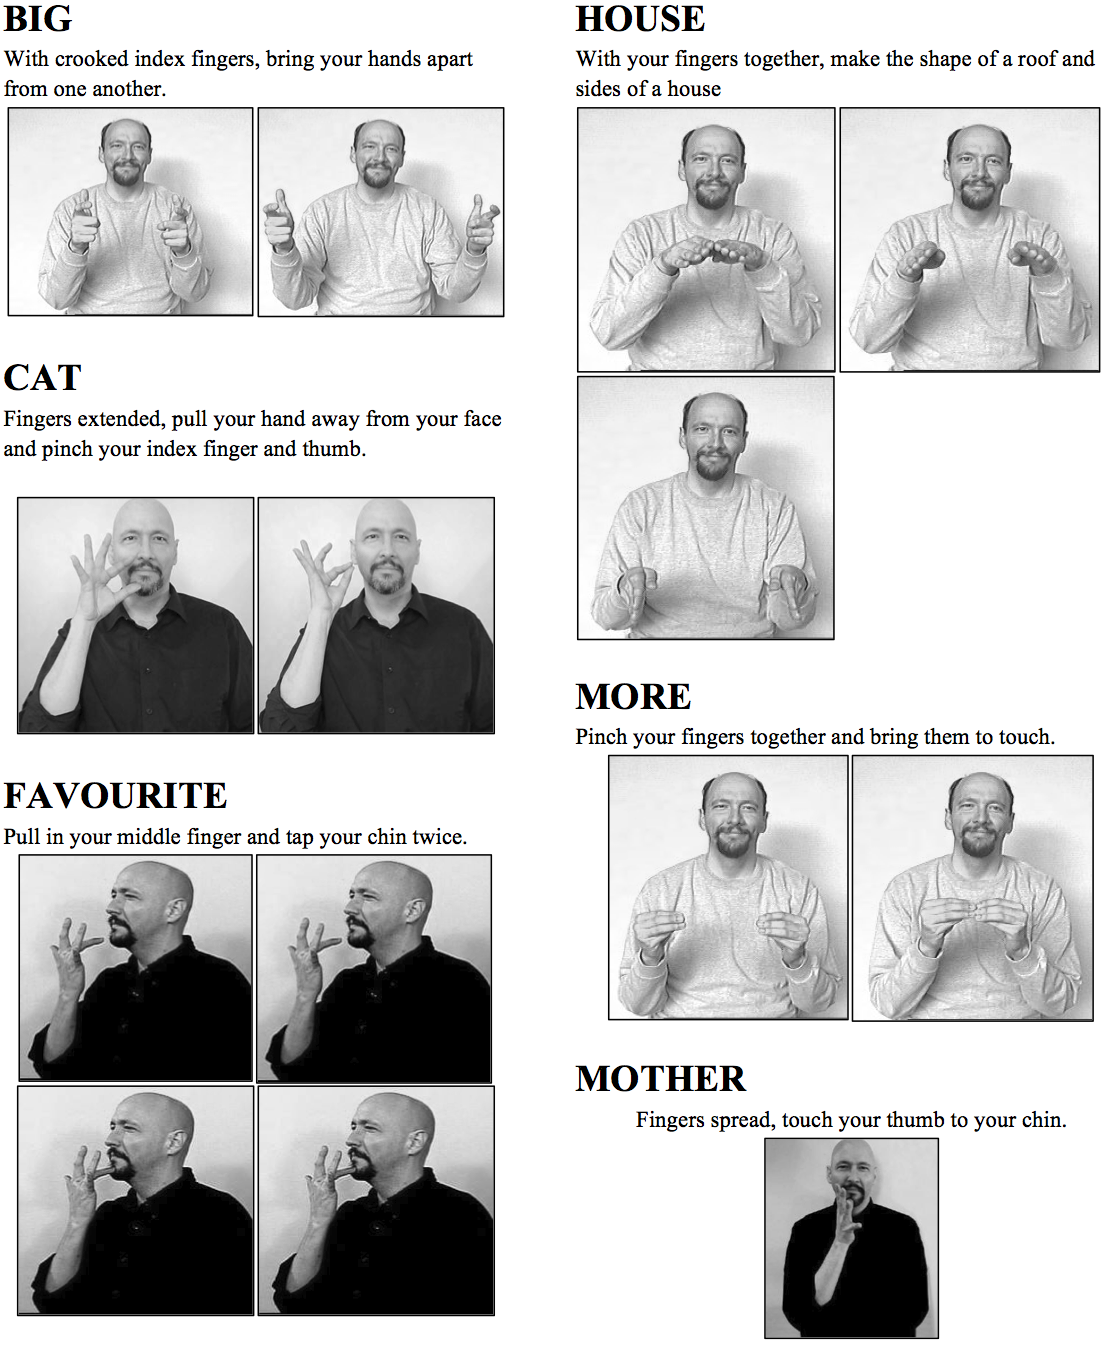
\includegraphics[scale=0.9]{signs1.png}
  \newpage
  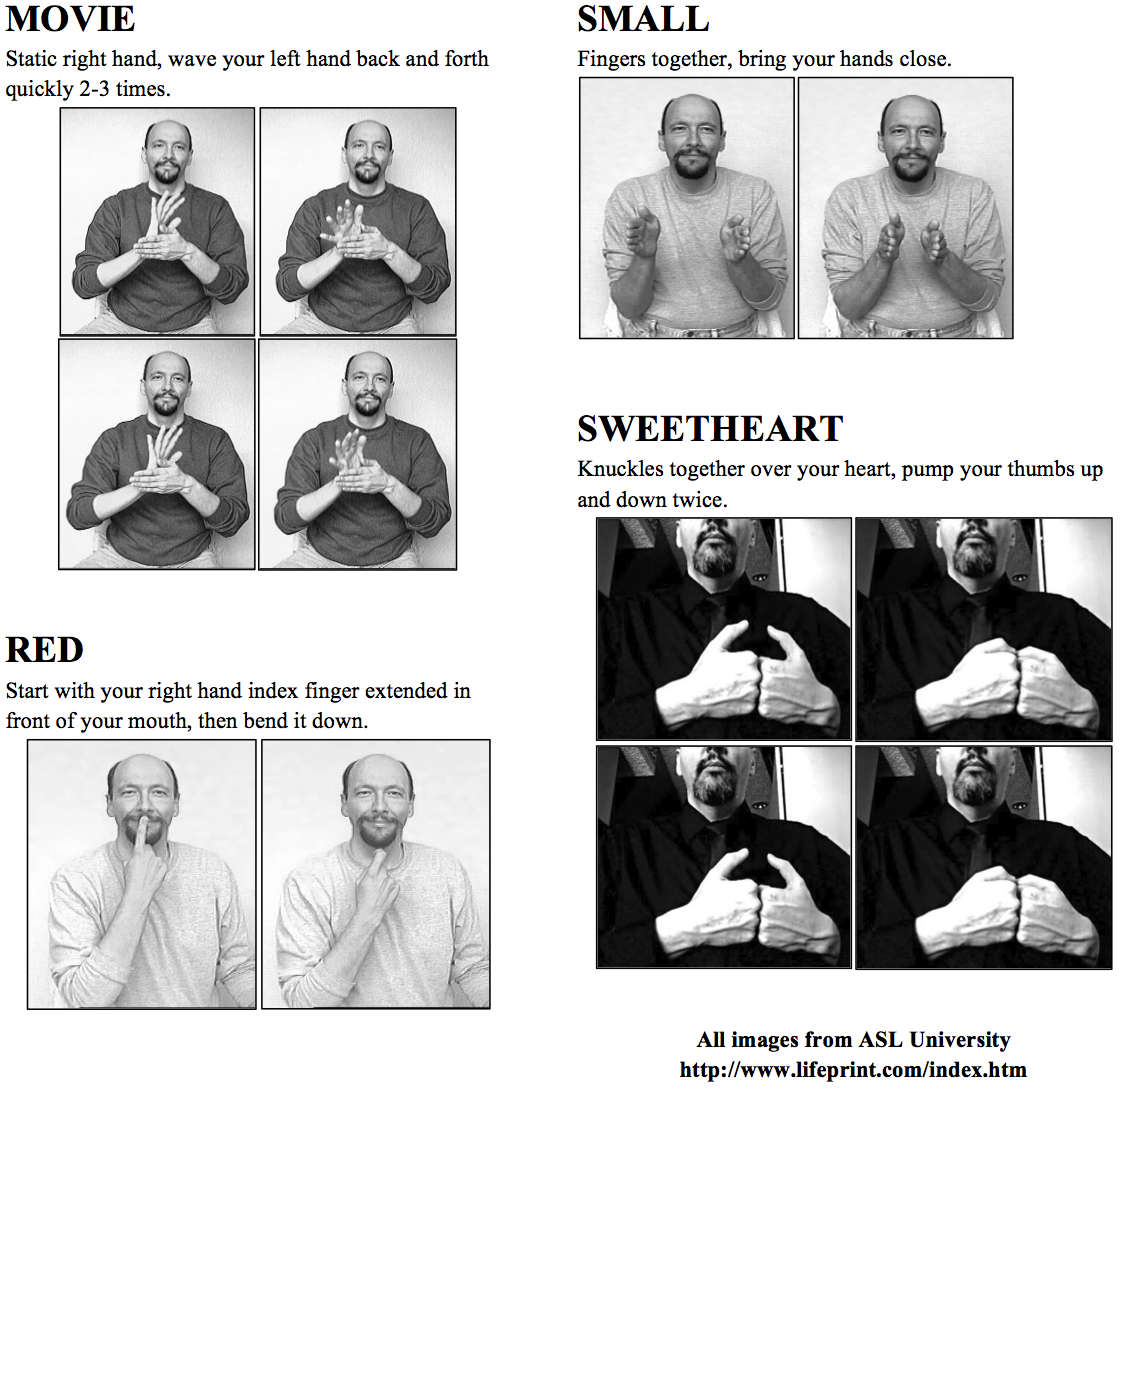
\includegraphics[scale=0.9]{signs2.png}


\newpage
\tocsection{Appendix B - Lighting Test Results}

\subsection*{Natural Light}
\subsubsection*{Trial 1}
\begin{table}[h]
\centering
\begin{tabular}{ll|c|c|c|c|c|c|c|c|c|c|c|c|}
\cline{3-14}
                               &                                  & \multicolumn{12}{c|}{Actual}                                                                                      \\ \cline{3-14} 
                               &                                  & \rotatebox[origin=c]{90}{BIG} & \rotatebox[origin=c]{90}{CAT} & \rotatebox[origin=c]{90}{  FAVOURITE  } & \rotatebox[origin=c]{90}{HOUSE} & \rotatebox[origin=c]{90}{MORE} & \rotatebox[origin=c]{90}{MOTHER} & \rotatebox[origin=c]{90}{MOVIE} & \rotatebox[origin=c]{90}{RED} & \rotatebox[origin=c]{90}{SMALL} & \rotatebox[origin=c]{90}{  SWEETHEART  } & \rotatebox[origin=c]{90}{  Not Recognized  } & \rotatebox[origin=c]{90}{  False Positive  }\\ \hline
\multicolumn{1}{|l}{}          & \multicolumn{1}{|l|}{BIG}        & 0   & 0   & 0         & 1     & 0    & 0      & 0     & 0   & 0     & 0          & 4              & 0              \\ \cline{2-14} 
\multicolumn{1}{|l}{}          & \multicolumn{1}{|l|}{CAT}        & 0   & 3   & 0         & 2     & 0    & 0      & 0     & 0   & 0     & 0          & 0              & 0              \\ \cline{2-14} 
\multicolumn{1}{|l}{}          & \multicolumn{1}{|l|}{FAVOURITE}  & 0   & 0   & 2         & 0     & 0    & 0      & 0     & 0   & 0     & 0          & 3              & 0              \\ \cline{2-14} 
\multicolumn{1}{|l}{}          & \multicolumn{1}{|l|}{HOUSE}      & 0   & 0   & 0         & 0     & 0    & 0      & 0     & 0   & 0     & 0          & 5              & 0              \\ \cline{2-14} 
\multicolumn{1}{|l}{Predicted} & \multicolumn{1}{|l|}{MORE}       & 0   & 0   & 0         & 0     & 5    & 0      & 0     & 0   & 0     & 0          & 0              & 0              \\ \cline{2-14} 
\multicolumn{1}{|l}{}          & \multicolumn{1}{|l|}{MOTHER}     & 0   & 0   & 0         & 0     & 0    & 5      & 0     & 0   & 0     & 0          & 0              & 0              \\ \cline{2-14} 
\multicolumn{1}{|l}{}          & \multicolumn{1}{|l|}{MOVIE}      & 5   & 0   & 0         & 0     & 0    & 0      & 0     & 0   & 0     & 0          & 0              & 0              \\ \cline{2-14} 
\multicolumn{1}{|l}{}          & \multicolumn{1}{|l|}{RED}        & 0   & 0   & 0         & 0     & 0    & 0      & 0     & 0   & 0     & 0          & 5              & 0              \\ \cline{2-14} 
\multicolumn{1}{|l}{}          & \multicolumn{1}{|l|}{SMALL}      & 0   & 0   & 0         & 0     & 0    & 0      & 0     & 0   & 2     & 0          & 3              & 0              \\ \cline{2-14} 
\multicolumn{1}{|l}{}          & \multicolumn{1}{|l|}{SWEETHEART} & 0   & 0   & 0         & 0     & 0    & 0      & 0     & 0   & 0     & 1          & 4              & 0              \\ \hline
\end{tabular}
\\
\begin{tabular}{l c}

\textbf{True Positives} & 18 \\
\textbf{Misclassifications} & 8 \\
\textbf{Not Recognized} & 24 \\
\textbf{False Positives} & 0 \\

\end{tabular}
\end{table}

\newpage
\subsubsection*{Trial 2}

\begin{table}[h]
\centering
\begin{tabular}{ll|l|l|l|l|l|l|l|l|l|l|l|l|}
\cline{3-14}
                      &                                  & \multicolumn{12}{c|}{Actual}                                                                                      \\ \cline{3-14} 
                               &                                  & \rotatebox[origin=c]{90}{BIG} & \rotatebox[origin=c]{90}{CAT} & \rotatebox[origin=c]{90}{  FAVOURITE  } & \rotatebox[origin=c]{90}{HOUSE} & \rotatebox[origin=c]{90}{MORE} & \rotatebox[origin=c]{90}{MOTHER} & \rotatebox[origin=c]{90}{MOVIE} & \rotatebox[origin=c]{90}{RED} & \rotatebox[origin=c]{90}{SMALL} & \rotatebox[origin=c]{90}{  SWEETHEART  } & \rotatebox[origin=c]{90}{  Not Recognized  } & \rotatebox[origin=c]{90}{  False Positive  }\\ \hline
\multicolumn{1}{|l}{} & \multicolumn{1}{|l|}{BIG}        & 1   & 0   & 0         & 1     & 0    & 0      & 0     & 0   & 0     & 0          & 3              & 0              \\ \cline{2-14} 
\multicolumn{1}{|l}{} & \multicolumn{1}{|l|}{CAT}        & 0   & 4   & 0         & 0     & 0    & 0      & 0     & 0   & 0     & 0          & 1              & 0              \\ \cline{2-14} 
\multicolumn{1}{|l}{} & \multicolumn{1}{|l|}{FAVOURITE}  & 0   & 2   & 0         & 0     & 0    & 0      & 0     & 0   & 0     & 0          & 3              & 0              \\ \cline{2-14} 
\multicolumn{1}{|l}{} & \multicolumn{1}{|l|}{HOUSE}      & 0   & 0   & 0         & 0     & 0    & 0      & 0     & 0   & 0     & 0          & 5              & 0              \\ \cline{2-14} 
\multicolumn{1}{|l}{Predicted} & \multicolumn{1}{|l|}{MORE}       & 0   & 0   & 0         & 0     & 3    & 0      & 0     & 0   & 0     & 0          & 2              & 0              \\ \cline{2-14} 
\multicolumn{1}{|l}{} & \multicolumn{1}{|l|}{MOTHER}     & 0   & 0   & 0         & 0     & 0    & 5      & 0     & 0   & 0     & 0          & 0              & 0              \\ \cline{2-14} 
\multicolumn{1}{|l}{} & \multicolumn{1}{|l|}{MOVIE}      & 0   & 0   & 0         & 0     & 0    & 0      & 4     & 0   & 0     & 0          & 1              & 0              \\ \cline{2-14} 
\multicolumn{1}{|l}{} & \multicolumn{1}{|l|}{RED}        & 0   & 0   & 0         & 0     & 0    & 0      & 0     & 1   & 0     & 0          & 4              & 0              \\ \cline{2-14} 
\multicolumn{1}{|l}{} & \multicolumn{1}{|l|}{SMALL}      & 0   & 0   & 0         & 0     & 0    & 0      & 0     & 0   & 5     & 0          & 0              & 0              \\ \cline{2-14} 
\multicolumn{1}{|l}{} & \multicolumn{1}{|l|}{SWEETHEART} & 0   & 0   & 0         & 0     & 0    & 0      & 0     & 0   & 0     & 5          & 0              & 0              \\ \hline
\end{tabular}
\\
\begin{tabular}{l c}

\textbf{True Positives} & 28 \\
\textbf{Misclassifications} & 3 \\
\textbf{Not Recognized} & 19 \\
\textbf{False Positives} & 0 \\

\end{tabular}
\end{table}

\newpage
\subsection*{Single Lamp}

\subsubsection*{Trial 1}
\begin{table}[h]
\centering
\begin{tabular}{ll|c|c|c|c|c|c|c|c|c|c|c|c|}
\cline{3-14}
                               &                                       & \multicolumn{12}{c|}{Actual}                                                                                \\ \cline{3-14} 
                               &                                  & \rotatebox[origin=c]{90}{BIG} & \rotatebox[origin=c]{90}{CAT} & \rotatebox[origin=c]{90}{  FAVOURITE  } & \rotatebox[origin=c]{90}{HOUSE} & \rotatebox[origin=c]{90}{MORE} & \rotatebox[origin=c]{90}{MOTHER} & \rotatebox[origin=c]{90}{MOVIE} & \rotatebox[origin=c]{90}{RED} & \rotatebox[origin=c]{90}{SMALL} & \rotatebox[origin=c]{90}{  SWEETHEART  } & \rotatebox[origin=c]{90}{  Not Recognized  } & \rotatebox[origin=c]{90}{  False Positive  }\\ \hline
\multicolumn{1}{|l}{}          & \multicolumn{1}{|l|}{BIG}        & 3   & 0   & 0         & 0     & 0    & 0      & 0     & 0   & 1     & 0          & 1              & 0              \\ \cline{2-14} 
\multicolumn{1}{|l}{}          & \multicolumn{1}{|l|}{CAT}        & 0   & 2   & 2         & 0     & 0    & 0      & 0     & 0   & 0     & 0          & 1              & 0              \\ \cline{2-14} 
\multicolumn{1}{|l}{}          & \multicolumn{1}{|l|}{FAVOURITE}  & 0   & 1   & 4         & 0     & 0    & 0      & 0     & 0   & 0     & 0          & 0              & 0              \\ \cline{2-14} 
\multicolumn{1}{|l}{}          & \multicolumn{1}{|l|}{HOUSE}      & 1   & 0   & 0         & 0     & 0    & 0      & 0     & 0   & 2     & 0          & 1              & 0              \\ \cline{2-14} 
\multicolumn{1}{|l}{Predicted} & \multicolumn{1}{|l|}{MORE}       & 0   & 0   & 0         & 0     & 5    & 0      & 0     & 0   & 0     & 0          & 0              & 0              \\ \cline{2-14} 
\multicolumn{1}{|l}{}          & \multicolumn{1}{|l|}{MOTHER}     & 0   & 0   & 0         & 0     & 0    & 4      & 0     & 0   & 0     & 0          & 1              & 0              \\ \cline{2-14} 
\multicolumn{1}{|l}{}          & \multicolumn{1}{|l|}{MOVIE}      & 1   & 0   & 0         & 0     & 0    & 0      & 4     & 0   & 0     & 0          & 0              & 0              \\ \cline{2-14} 
\multicolumn{1}{|l}{}          & \multicolumn{1}{|l|}{RED}        & 0   & 2   & 0         & 0     & 0    & 0      & 0     & 0   & 0     & 0          & 3              & 0              \\ \cline{2-14} 
\multicolumn{1}{|l}{}          & \multicolumn{1}{|l|}{SMALL}      & 0   & 0   & 0         & 0     & 0    & 0      & 0     & 0   & 4     & 0          & 1              & 0              \\ \cline{2-14} 
\multicolumn{1}{|l}{}          & \multicolumn{1}{|l|}{SWEETHEART} & 0   & 0   & 0         & 0     & 0    & 0      & 0     & 0   & 0     & 4          & 1              & 0              \\ \hline
\end{tabular}
\\
\begin{tabular}{l c}

\textbf{True Positives} & 30 \\
\textbf{Misclassifications} & 10 \\
\textbf{Not Recognized} & 10 \\
\textbf{False Positives} & 0 \\

\end{tabular}
\end{table}

\newpage
\subsubsection*{Trial 2}
\begin{table}[h]
\centering
\begin{tabular}{ll|c|c|c|c|c|c|c|c|c|c|c|c|}
\cline{3-14}
                               &                                  & \multicolumn{12}{c|}{Actual}                                                                                            \\ \cline{3-14} 
                               &                                  & \rotatebox[origin=c]{90}{BIG} & \rotatebox[origin=c]{90}{CAT} & \rotatebox[origin=c]{90}{  FAVOURITE  } & \rotatebox[origin=c]{90}{HOUSE} & \rotatebox[origin=c]{90}{MORE} & \rotatebox[origin=c]{90}{MOTHER} & \rotatebox[origin=c]{90}{MOVIE} & \rotatebox[origin=c]{90}{RED} & \rotatebox[origin=c]{90}{SMALL} & \rotatebox[origin=c]{90}{  SWEETHEART  } & \rotatebox[origin=c]{90}{  Not Recognized  } & \rotatebox[origin=c]{90}{  False Positive  }\\ \hline
\multicolumn{1}{|l}{}          & \multicolumn{1}{|l|}{BIG}        & 0   & 0   & 0         & 1     & 0    & 0      & 0     & 0   & 0     & 0          & 4              & 0              \\ \cline{2-14} 
\multicolumn{1}{|l}{}          & \multicolumn{1}{|l|}{CAT}        & 0   & 4   & 0         & 0     & 0    & 0      & 0     & 0   & 0     & 0          & 1              & 0              \\ \cline{2-14} 
\multicolumn{1}{|l}{}          & \multicolumn{1}{|l|}{FAVOURITE}  & 0   & 0   & 5         & 0     & 0    & 0      & 0     & 0   & 0     & 0          & 0              & 0              \\ \cline{2-14} 
\multicolumn{1}{|l}{}          & \multicolumn{1}{|l|}{HOUSE}      & 0   & 0   & 0         & 2     & 0    & 0      & 0     & 0   & 0     & 0          & 3              & 0              \\ \cline{2-14} 
\multicolumn{1}{|l}{Predicted} & \multicolumn{1}{|l|}{MORE}       & 0   & 0   & 0         & 0     & 3    & 0      & 0     & 0   & 1     & 0          & 1              & 0              \\ \cline{2-14} 
\multicolumn{1}{|l}{}          & \multicolumn{1}{|l|}{MOTHER}     & 0   & 0   & 0         & 0     & 0    & 0      & 0     & 0   & 3     & 0          & 2              & 0              \\ \cline{2-14} 
\multicolumn{1}{|l}{}          & \multicolumn{1}{|l|}{MOVIE}      & 0   & 0   & 0         & 0     & 0    & 0      & 3     & 0   & 0     & 0          & 2              & 0              \\ \cline{2-14} 
\multicolumn{1}{|l}{}          & \multicolumn{1}{|l|}{RED}        & 0   & 0   & 0         & 0     & 0    & 0      & 0     & 2   & 0     & 0          & 3              & 0              \\ \cline{2-14} 
\multicolumn{1}{|l}{}          & \multicolumn{1}{|l|}{SMALL}      & 0   & 0   & 0         & 0     & 0    & 0      & 0     & 0   & 3     & 0          & 2              & 0              \\ \cline{2-14} 
\multicolumn{1}{|l}{}          & \multicolumn{1}{|l|}{SWEETHEART} & 0   & 0   & 0         & 0     & 0    & 0      & 0     & 0   & 0     & 4          & 1              & 0              \\ \hline
\end{tabular}
\\
\begin{tabular}{l c}

\textbf{True Positives} & 26 \\
\textbf{Misclassifications} & 5 \\
\textbf{Not Recognized} & 19 \\
\textbf{False Positives} & 0 \\

\end{tabular}
\end{table}

\newpage
\subsection*{Ambient Light}

\subsubsection*{Trial 1}
\begin{table}[h]
\centering
\begin{tabular}{ll|c|c|c|c|c|c|c|c|c|c|c|c|}
\cline{3-14}
                               &                                  & \multicolumn{12}{c|}{Actual}                                                                                      \\ \cline{3-14} 
                               &                                  & \rotatebox[origin=c]{90}{BIG} & \rotatebox[origin=c]{90}{CAT} & \rotatebox[origin=c]{90}{  FAVOURITE  } & \rotatebox[origin=c]{90}{HOUSE} & \rotatebox[origin=c]{90}{MORE} & \rotatebox[origin=c]{90}{MOTHER} & \rotatebox[origin=c]{90}{MOVIE} & \rotatebox[origin=c]{90}{RED} & \rotatebox[origin=c]{90}{SMALL} & \rotatebox[origin=c]{90}{  SWEETHEART  } & \rotatebox[origin=c]{90}{  Not Recognized  } & \rotatebox[origin=c]{90}{  False Positive  }\\ \hline
\multicolumn{1}{|l}{}          & \multicolumn{1}{|l|}{BIG}        & 0   & 0   & 0         & 0     & 0    & 0      & 0     & 0   & 0     & 0          & 5              & 0              \\ \cline{2-14} 
\multicolumn{1}{|l}{}          & \multicolumn{1}{|l|}{CAT}        & 0   & 5   & 0         & 0     & 0    & 0      & 0     & 0   & 0     & 0          & 0              & 0              \\ \cline{2-14} 
\multicolumn{1}{|l}{}          & \multicolumn{1}{|l|}{FAVOURITE}  & 0   & 0   & 4         & 0     & 0    & 0      & 0     & 0   & 0     & 0          & 1              & 0              \\ \cline{2-14} 
\multicolumn{1}{|l}{}          & \multicolumn{1}{|l|}{HOUSE}      & 1   & 0   & 0         & 1     & 0    & 0      & 0     & 0   & 0     & 0          & 3              & 0              \\ \cline{2-14} 
\multicolumn{1}{|l}{Predicted} & \multicolumn{1}{|l|}{MORE}       & 0   & 0   & 0         & 0     & 4    & 0      & 0     & 0   & 0     & 0          & 1              & 0              \\ \cline{2-14} 
\multicolumn{1}{|l}{}          & \multicolumn{1}{|l|}{MOTHER}     & 0   & 0   & 0         & 0     & 0    & 5      & 0     & 0   & 0     & 0          & 0              & 0              \\ \cline{2-14} 
\multicolumn{1}{|l}{}          & \multicolumn{1}{|l|}{MOVIE}      & 0   & 0   & 0         & 0     & 0    & 0      & 5     & 0   & 0     & 0          & 0              & 0              \\ \cline{2-14} 
\multicolumn{1}{|l}{}          & \multicolumn{1}{|l|}{RED}        & 2   & 0   & 0         & 0     & 0    & 0      & 0     & 0   & 0     & 0          & 3              & 0              \\ \cline{2-14} 
\multicolumn{1}{|l}{}          & \multicolumn{1}{|l|}{SMALL}      & 0   & 0   & 0         & 0     & 0    & 0      & 0     & 0   & 5     & 0          & 0              & 0              \\ \cline{2-14} 
\multicolumn{1}{|l}{}          & \multicolumn{1}{|l|}{SWEETHEART} & 1   & 0   & 0         & 0     & 0    & 0      & 0     & 0   & 0     & 4          & 0              & 0              \\ \hline
\end{tabular}
\\
\begin{tabular}{l c}

\textbf{True Positives} & 33 \\
\textbf{Misclassifications} & 4 \\
\textbf{Not Recognized} & 13 \\
\textbf{False Positives} & 0 \\

\end{tabular}
\end{table}

\newpage
\subsubsection*{Trial 2}

\begin{table}[h]
\centering
\begin{tabular}{ll|c|c|c|c|c|c|c|c|c|c|c|c|}
\cline{3-14}
                               &                                  & \multicolumn{12}{c|}{Actual}                                                                                      \\ \cline{3-14} 
                               &                                  & \rotatebox[origin=c]{90}{BIG} & \rotatebox[origin=c]{90}{CAT} & \rotatebox[origin=c]{90}{  FAVOURITE  } & \rotatebox[origin=c]{90}{HOUSE} & \rotatebox[origin=c]{90}{MORE} & \rotatebox[origin=c]{90}{MOTHER} & \rotatebox[origin=c]{90}{MOVIE} & \rotatebox[origin=c]{90}{RED} & \rotatebox[origin=c]{90}{SMALL} & \rotatebox[origin=c]{90}{  SWEETHEART  } & \rotatebox[origin=c]{90}{  Not Recognized  } & \rotatebox[origin=c]{90}{  False Positive  }\\ \hline
\multicolumn{1}{|l}{}          & \multicolumn{1}{|l|}{BIG}        & 1   & 0   & 0         & 0     & 0    & 0      & 0     & 0   & 0     & 0          & 4              & 0              \\ \cline{2-14} 
\multicolumn{1}{|l}{}          & \multicolumn{1}{|l|}{CAT}        & 0   & 5   & 0         & 0     & 0    & 0      & 0     & 0   & 0     & 0          & 0              & 0              \\ \cline{2-14} 
\multicolumn{1}{|l}{}          & \multicolumn{1}{|l|}{FAVOURITE}  & 0   & 0   & 5         & 0     & 0    & 0      & 0     & 0   & 0     & 0          & 0              & 0              \\ \cline{2-14} 
\multicolumn{1}{|l}{}          & \multicolumn{1}{|l|}{HOUSE}      & 0   & 0   & 0         & 2     & 0    & 0      & 0     & 0   & 0     & 0          & 3              & 0              \\ \cline{2-14} 
\multicolumn{1}{|l}{Predicted} & \multicolumn{1}{|l|}{MORE}       & 0   & 0   & 0         & 0     & 4    & 0      & 0     & 0   & 0     & 0          & 1              & 0              \\ \cline{2-14} 
\multicolumn{1}{|l}{}          & \multicolumn{1}{|l|}{MOTHER}     & 0   & 0   & 0         & 0     & 0    & 5      & 0     & 0   & 0     & 0          & 0              & 0              \\ \cline{2-14} 
\multicolumn{1}{|l}{}          & \multicolumn{1}{|l|}{MOVIE}      & 0   & 0   & 0         & 0     & 0    & 0      & 5     & 0   & 0     & 0          & 0              & 0              \\ \cline{2-14} 
\multicolumn{1}{|l}{}          & \multicolumn{1}{|l|}{RED}        & 0   & 0   & 0         & 0     & 0    & 0      & 0     & 2   & 0     & 0          & 3              & 0              \\ \cline{2-14} 
\multicolumn{1}{|l}{}          & \multicolumn{1}{|l|}{SMALL}      & 0   & 0   & 0         & 0     & 0    & 0      & 0     & 0   & 5     & 0          & 0              & 0              \\ \cline{2-14} 
\multicolumn{1}{|l}{}          & \multicolumn{1}{|l|}{SWEETHEART} & 2   & 0   & 0         & 0     & 0    & 0      & 0     & 0   & 0     & 3          & 0              & 0              \\ \hline
\end{tabular}
\\
\begin{tabular}{l c}

\textbf{True Positives} & 37 \\
\textbf{Misclassifications} & 2 \\
\textbf{Not Recognized} & 11 \\
\textbf{False Positives} & 0 \\

\end{tabular}
\end{table}

\end{document}